\documentclass[tikz,border=8pt]{standalone}
\usepackage{amsmath}
\usepackage{amssymb}
\usetikzlibrary{arrows.meta,calc,positioning}

\definecolor{basisblue}{HTML}{2F6F9F}
\definecolor{basisgreen}{HTML}{5F7F55}
\definecolor{basisgold}{HTML}{A66F00}
\definecolor{textgray}{HTML}{2F3437}
\definecolor{linegray}{HTML}{AEB7BC}
\definecolor{softgray}{HTML}{F5F7F8}

\begin{document}
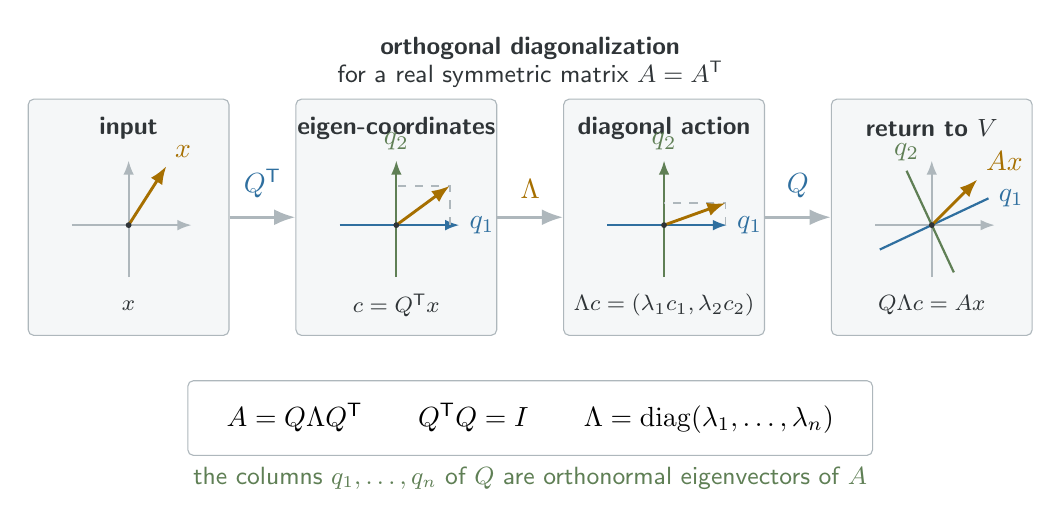
\begin{tikzpicture}[
  font=\sffamily,
  >=Latex,
  vector/.style={-{Latex[length=2.3mm]}, line width=1.05pt},
  axis/.style={-{Latex[length=1.8mm]}, draw=linegray, line width=0.7pt},
  maparrow/.style={-{Latex[length=2.7mm]}, draw=linegray, line width=1.0pt},
  guide/.style={draw=linegray, dashed, line width=0.65pt},
  panel/.style={
    draw=linegray,
    fill=softgray,
    rounded corners=2pt,
    minimum width=2.55cm,
    minimum height=3.0cm
  },
  stage/.style={
    draw=linegray,
    fill=white,
    rounded corners=2pt,
    inner xsep=14pt,
    inner ysep=8pt,
    align=center
  },
  label/.style={font=\sffamily\bfseries\small, text=textgray},
  smallnote/.style={font=\sffamily\small, text=textgray, align=center},
  mathnote/.style={font=\sffamily\footnotesize, text=textgray, align=center}
]

\node[label] at (0,2.15) {orthogonal diagonalization};
\node[smallnote] at (0,1.82) {for a real symmetric matrix $A=A^{\mathsf T}$};

% Four stages of A x = Q Lambda Q^T x.
\node[panel] (input) at (-5.10,0) {};
\node[panel] (coords) at (-1.70,0) {};
\node[panel] (scale) at (1.70,0) {};
\node[panel] (output) at (5.10,0) {};

\node[label] at (-5.10,1.13) {input};
\node[label] at (-1.70,1.13) {eigen-coordinates};
\node[label] at (1.70,1.13) {diagonal action};
\node[label] at (5.10,1.13) {return to $V$};

% Input vector in the original coordinates.
\begin{scope}[shift={(-5.10,-0.10)}]
  \draw[axis] (-0.72,0) -- (0.80,0);
  \draw[axis] (0,-0.66) -- (0,0.82);
  \draw[vector, draw=basisgold] (0,0) -- (0.48,0.75)
    node[above right=-1pt, text=basisgold] {$x$};
  \fill[textgray] (0,0) circle (1.05pt);
\end{scope}
\node[mathnote] at (-5.10,-1.12) {$x$};

% Coordinates c_i = <q_i,x> in the orthonormal eigenbasis.
\begin{scope}[shift={(-1.70,-0.10)}]
  \draw[axis, draw=basisblue] (-0.72,0) -- (0.80,0)
    node[right, text=basisblue] {$q_1$};
  \draw[axis, draw=basisgreen] (0,-0.66) -- (0,0.82)
    node[above, text=basisgreen] {$q_2$};
  \draw[guide] (0.68,0) -- (0.68,0.50) -- (0,0.50);
  \draw[vector, draw=basisgold] (0,0) -- (0.68,0.50);
  \fill[textgray] (0,0) circle (1.05pt);
\end{scope}
\node[mathnote] at (-1.70,-1.12) {$c=Q^{\mathsf T}x$};

% Lambda acts independently on the eigen-coordinates.
\begin{scope}[shift={(1.70,-0.10)}]
  \draw[axis, draw=basisblue] (-0.72,0) -- (0.80,0)
    node[right, text=basisblue] {$q_1$};
  \draw[axis, draw=basisgreen] (0,-0.66) -- (0,0.82)
    node[above, text=basisgreen] {$q_2$};
  \draw[guide] (0.78,0) -- (0.78,0.28) -- (0,0.28);
  \draw[vector, draw=basisgold] (0,0) -- (0.78,0.28);
  \fill[textgray] (0,0) circle (1.05pt);
\end{scope}
\node[mathnote] at (1.70,-1.12)
  {$\Lambda c=(\lambda_1c_1,\lambda_2c_2)$};

% Q rotates/reflections the scaled coordinates back to V.
\begin{scope}[shift={(5.10,-0.10)}]
  \draw[axis] (-0.72,0) -- (0.80,0);
  \draw[axis] (0,-0.66) -- (0,0.82);
  \draw[draw=basisblue, line width=0.8pt]
    (-0.66,-0.31) -- (0.72,0.34)
    node[right, text=basisblue] {$q_1$};
  \draw[draw=basisgreen, line width=0.8pt]
    (0.28,-0.60) -- (-0.32,0.69)
    node[above, text=basisgreen] {$q_2$};
  \draw[vector, draw=basisgold] (0,0) -- (0.58,0.58)
    node[above right=-1pt, text=basisgold] {$Ax$};
  \fill[textgray] (0,0) circle (1.05pt);
\end{scope}
\node[mathnote] at (5.10,-1.12) {$Q\Lambda c=Ax$};

% Change basis, scale, and change back.
\draw[maparrow] (input.east) -- (coords.west)
  node[midway, above=3pt, text=basisblue] {$Q^{\mathsf T}$};
\draw[maparrow] (coords.east) -- (scale.west)
  node[midway, above=3pt, text=basisgold] {$\Lambda$};
\draw[maparrow] (scale.east) -- (output.west)
  node[midway, above=3pt, text=basisblue] {$Q$};

% Algebraic summary.
\node[stage, minimum width=6.25cm] at (0,-2.55)
  {$A=Q\Lambda Q^{\mathsf T}$\qquad
   $Q^{\mathsf T}Q=I$\qquad
   $\Lambda=\operatorname{diag}(\lambda_1,\ldots,\lambda_n)$};

\node[smallnote, text=basisgreen] at (0,-3.32)
  {the columns $q_1,\ldots,q_n$ of $Q$ are orthonormal eigenvectors of $A$};

\end{tikzpicture}
\end{document}
